
\section{Expansion-Ratio Selection and Ideal Performance Mapping}
% =========================================================

\subsection{Ideal operating-point and performance maps}

\subsubsection{Ambient-pressure matching and expansion-ratio search}

For a given chamber pressure, mixture ratio and propellant combination, the simulator can estimate the expansion ratio that best matches the desired ambient pressure. The ideal criterion is
\begin{equation}
p_e(\varepsilon)=p_a.
\label{eq:epsilon_target}
\end{equation}

The numerical search evaluates the exit pressure for a range of expansion ratios and selects the value that minimizes
\begin{equation}
E_{\varepsilon}=\left|p_e(\varepsilon)-p_a\right|.
\label{eq:epsilon_error}
\end{equation}

If the search is performed for several chamber pressures, the result can be plotted as an ideal expansion-ratio curve. Interpolation may then be used to estimate an appropriate $\varepsilon$ for intermediate chamber pressures.

\begin{figure}[H]
    \centering
    \IfFileExists{Images/ex19.png}{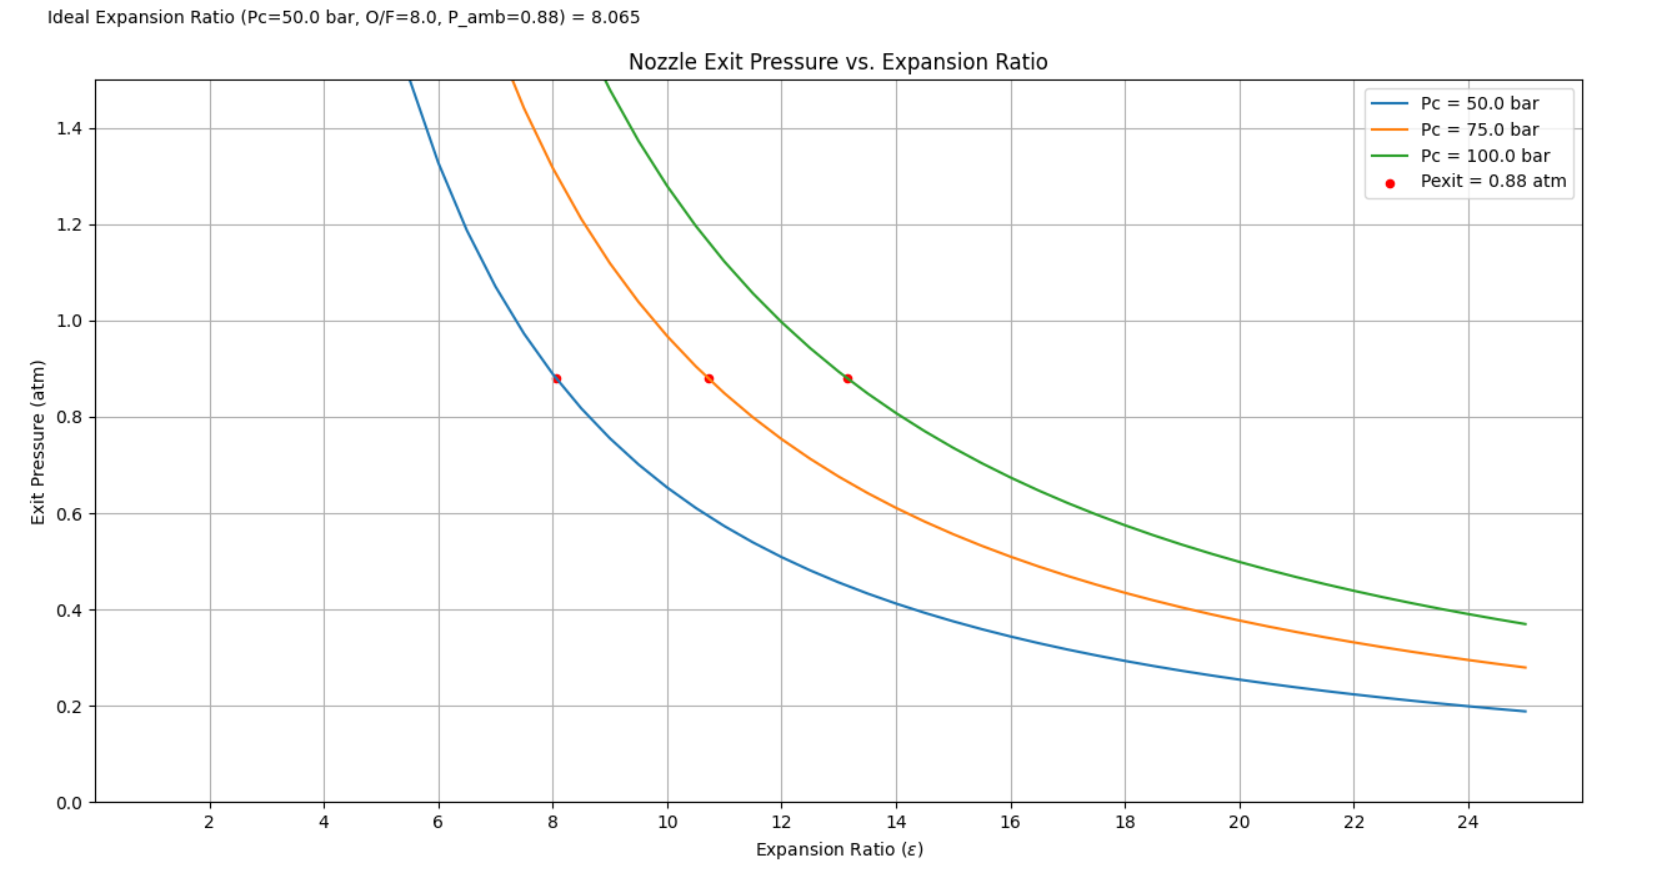
\includegraphics[width=0.82\linewidth]{Images/ex19.png}}{\fbox{\parbox{0.82\linewidth}{\centering Missing figure file: \texttt{ex19.png}}}}
    \caption{Example output for ideal expansion ratio estimation.}
    \label{fig:ideal_expansion_result}
\end{figure}

\subsubsection{Exit velocity and exit-temperature evaluation}

Under the ideal isentropic model, the exhaust velocity can be estimated from the chamber temperature and exit temperature:
\begin{equation}
V_e=\sqrt{\frac{2\gamma}{\gamma-1}RT_0\left[1-\left(\frac{p_e}{p_0}\right)^{(\gamma-1)/\gamma}\right]}.
\label{eq:ve_pressure}
\end{equation}

Equivalently, once the exit Mach number is known,
\begin{equation}
V_e=M_e\sqrt{\gamma R T_e}.
\label{eq:ve_mach}
\end{equation}

The exit temperature is obtained from Eq.~\eqref{eq:T_T0}:
\begin{equation}
T_e=\frac{T_0}{1+\dfrac{\gamma-1}{2}M_e^2}.
\label{eq:Te}
\end{equation}

The simulator can therefore plot exhaust velocity and exhaust temperature as functions of chamber pressure, expansion ratio or mixture ratio. These plots help identify the sensitivity of nozzle performance to the operating point.

\begin{figure}[H]
    \centering
    \begin{subfigure}{0.48\linewidth}
        \centering
        \IfFileExists{Images/ex20.png}{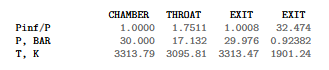
\includegraphics[width=\linewidth]{Images/ex20.png}}{\fbox{\parbox{0.95\linewidth}{\centering Missing: \texttt{ex20.png}}}}
        \caption{Example exhaust velocity trend.}
    \end{subfigure}
    \hfill
    \begin{subfigure}{0.48\linewidth}
        \centering
        \IfFileExists{Images/ex21.png}{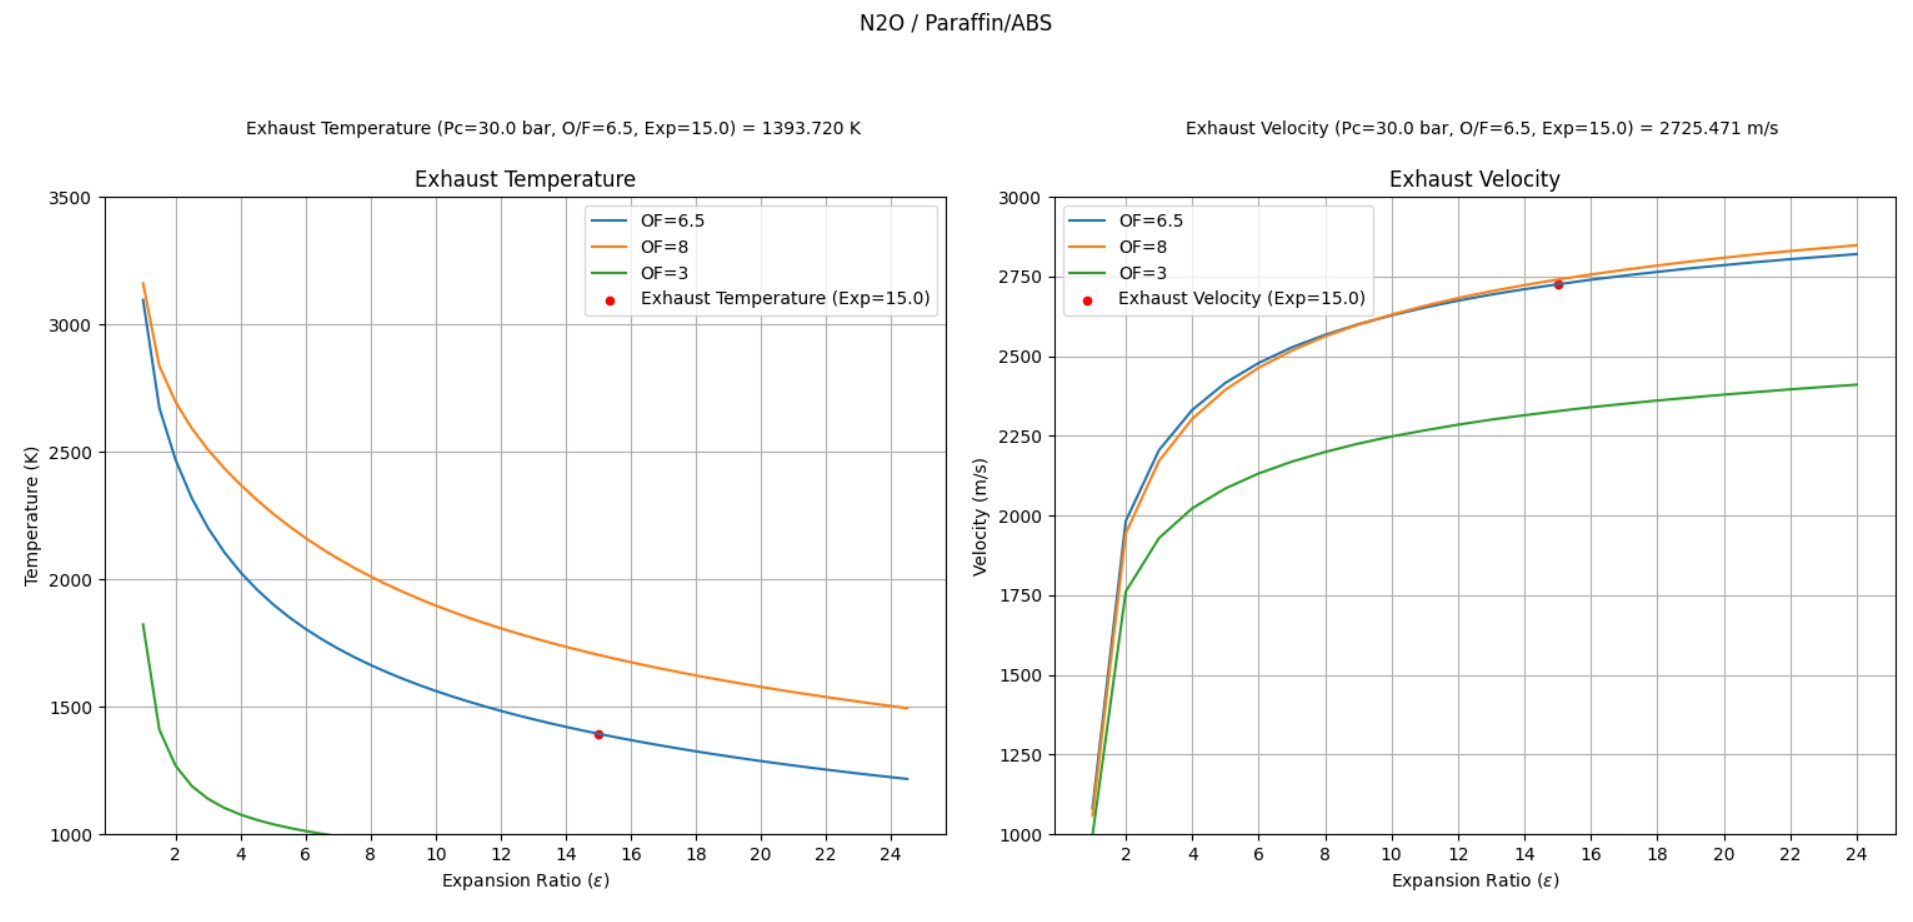
\includegraphics[width=\linewidth]{Images/ex21.png}}{\fbox{\parbox{0.95\linewidth}{\centering Missing: \texttt{ex21.png}}}}
        \caption{Example exhaust temperature trend.}
    \end{subfigure}
    \caption{Example performance plots generated by the simulator.}
    \label{fig:exhaust_plots}
\end{figure}

\subsubsection{Thrust coefficient, characteristic velocity and specific impulse}

The main ideal performance parameters are:
\begin{align}
I_{sp} &= \frac{F}{\dot{m}g_0},
\label{eq:Isp}\\
c^* &= \frac{p_c A_t}{\dot{m}},
\label{eq:cstar}\\
C_F &= \frac{F}{p_c A_t}.
\label{eq:CF}
\end{align}

The characteristic velocity $c^*$ mainly measures combustion and thermochemical performance, while the thrust coefficient $C_F$ measures how effectively the nozzle converts chamber pressure into thrust. The specific impulse $I_{sp}$ combines the full propulsion performance into an impulse per unit propellant weight flow.

\begin{figure}[H]
    \centering
    \IfFileExists{Images/ex23.png}{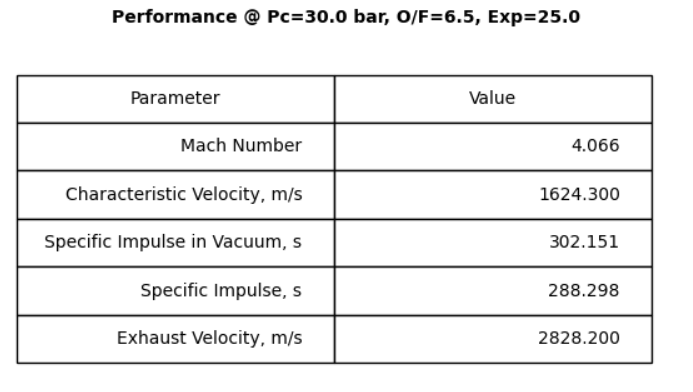
\includegraphics[width=0.82\linewidth]{Images/ex23.png}}{\fbox{\parbox{0.82\linewidth}{\centering Missing figure file: \texttt{Images/ex23.png}}}}
    \caption{Example performance-parameter output table and plot.}
    \label{fig:performance_parameters}
\end{figure}